\chapter{UML diagramy}
\section{Use cases}

\begin{figure}[h]
\begin{center}
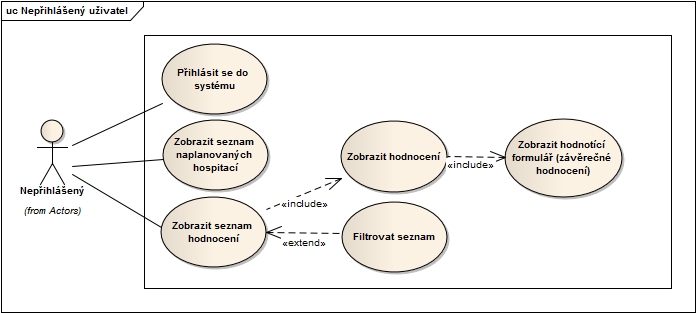
\includegraphics[width=12cm]{figures/actor_base}
\caption{Use case - nepřihlášený uživatel}
\label{fig:actor_base}
\end{center}
\end{figure}

\begin{figure}[h]
\begin{center}
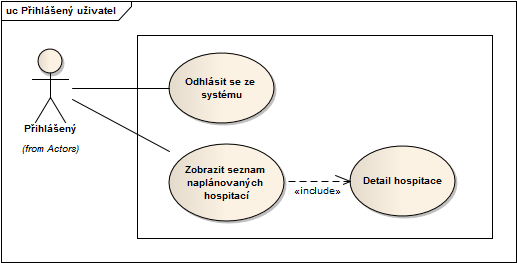
\includegraphics[width=12cm]{figures/actor_logged}
\caption{Use case - přihlášený uživatel}
\label{fig:actor_logged}
\end{center}
\end{figure}

\begin{figure}[h]
\begin{center}
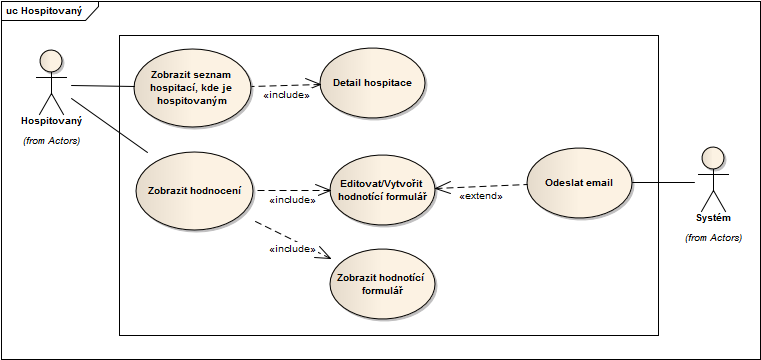
\includegraphics[width=12cm]{figures/actor_observed}
\caption{Use case - hospitovaný}
\label{fig:actor_observed}
\end{center}
\end{figure}

\begin{figure}[h]
\begin{center}
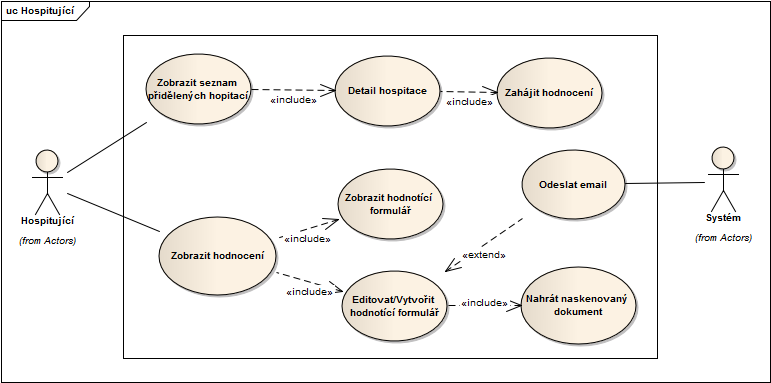
\includegraphics[width=12cm]{figures/actor_observer}
\caption{Use case - hospitující}
\label{fig:actor_observer}
\end{center}
\end{figure}

\begin{figure}[h]
\begin{center}
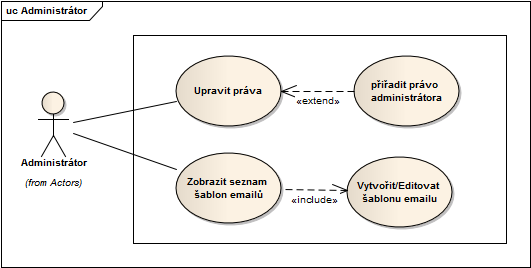
\includegraphics[width=12cm]{figures/actor_root}
\caption{Use case - administrátor}
\label{fig:actor_root}
\end{center}
\end{figure}

\begin{figure}[h]
\begin{center}
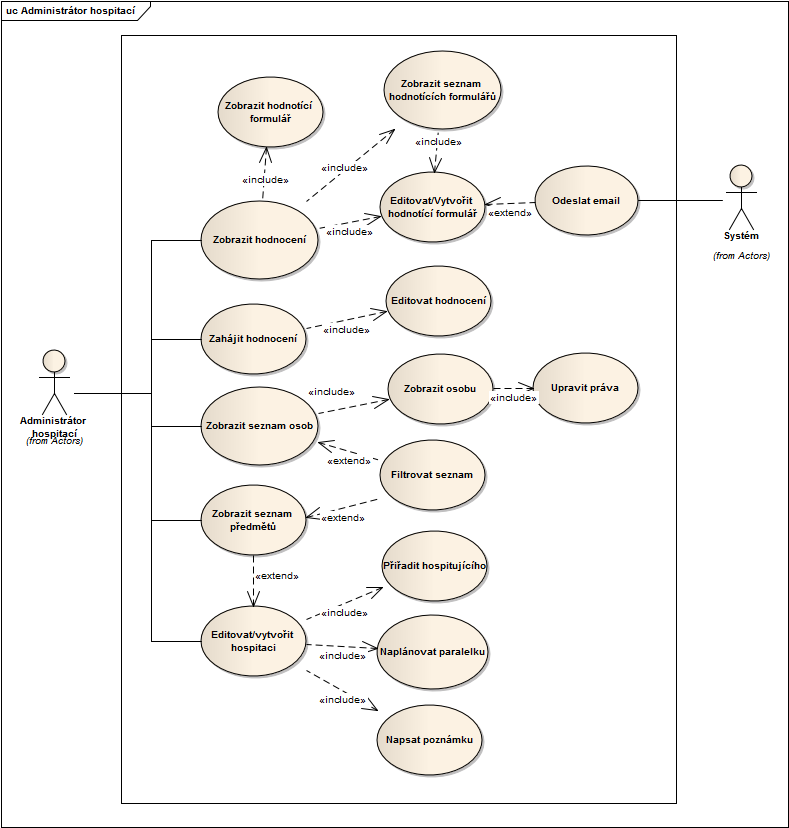
\includegraphics[width=14cm]{figures/actor_admin}
\caption{Use case - administrátor hospitací}
\label{fig:actor_admin}
\end{center}
\end{figure}

